\documentclass{beamer}
\usetheme{metropolis}           % Use metropolis theme
\title{Machine learning im Bereich der Robotik}
\date{\today}
\author{Robin Eberhard}

\begin{document}
  \maketitle
  \begin{frame}{Pancakes machen}
  \begin{center}
  	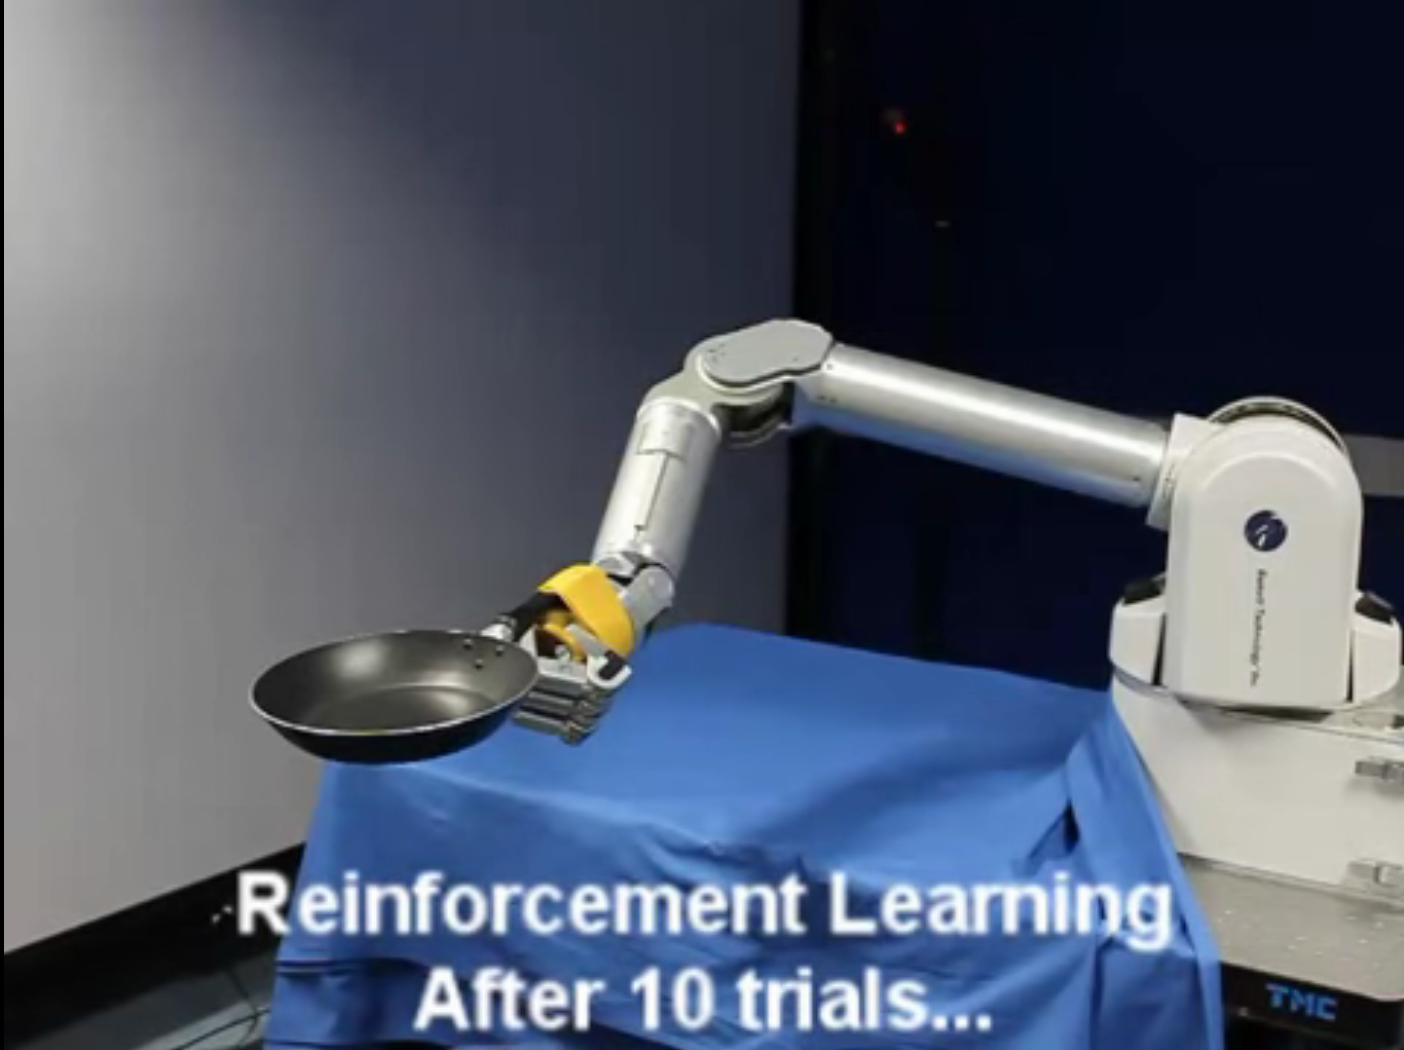
\includegraphics[scale=0.15]{img/pancake.png} \\
  	\url{https://youtu.be/W_gxLKSsSIE?t=51}
  \end{center}
  \end{frame}
  
  %%%%%%%%%%%%%%%%%%%%%%%%%%%%%%%%%%%%%%%%%%%%%%%%
  %%%%%%%%% Quadrotor %%%%%%%%%%%%%%%%%%%%%%%%%%%%
  \section{Quadrotor im Wald}
  \begin{frame}{Quadrotor im Wald}
  \begin{center}
  	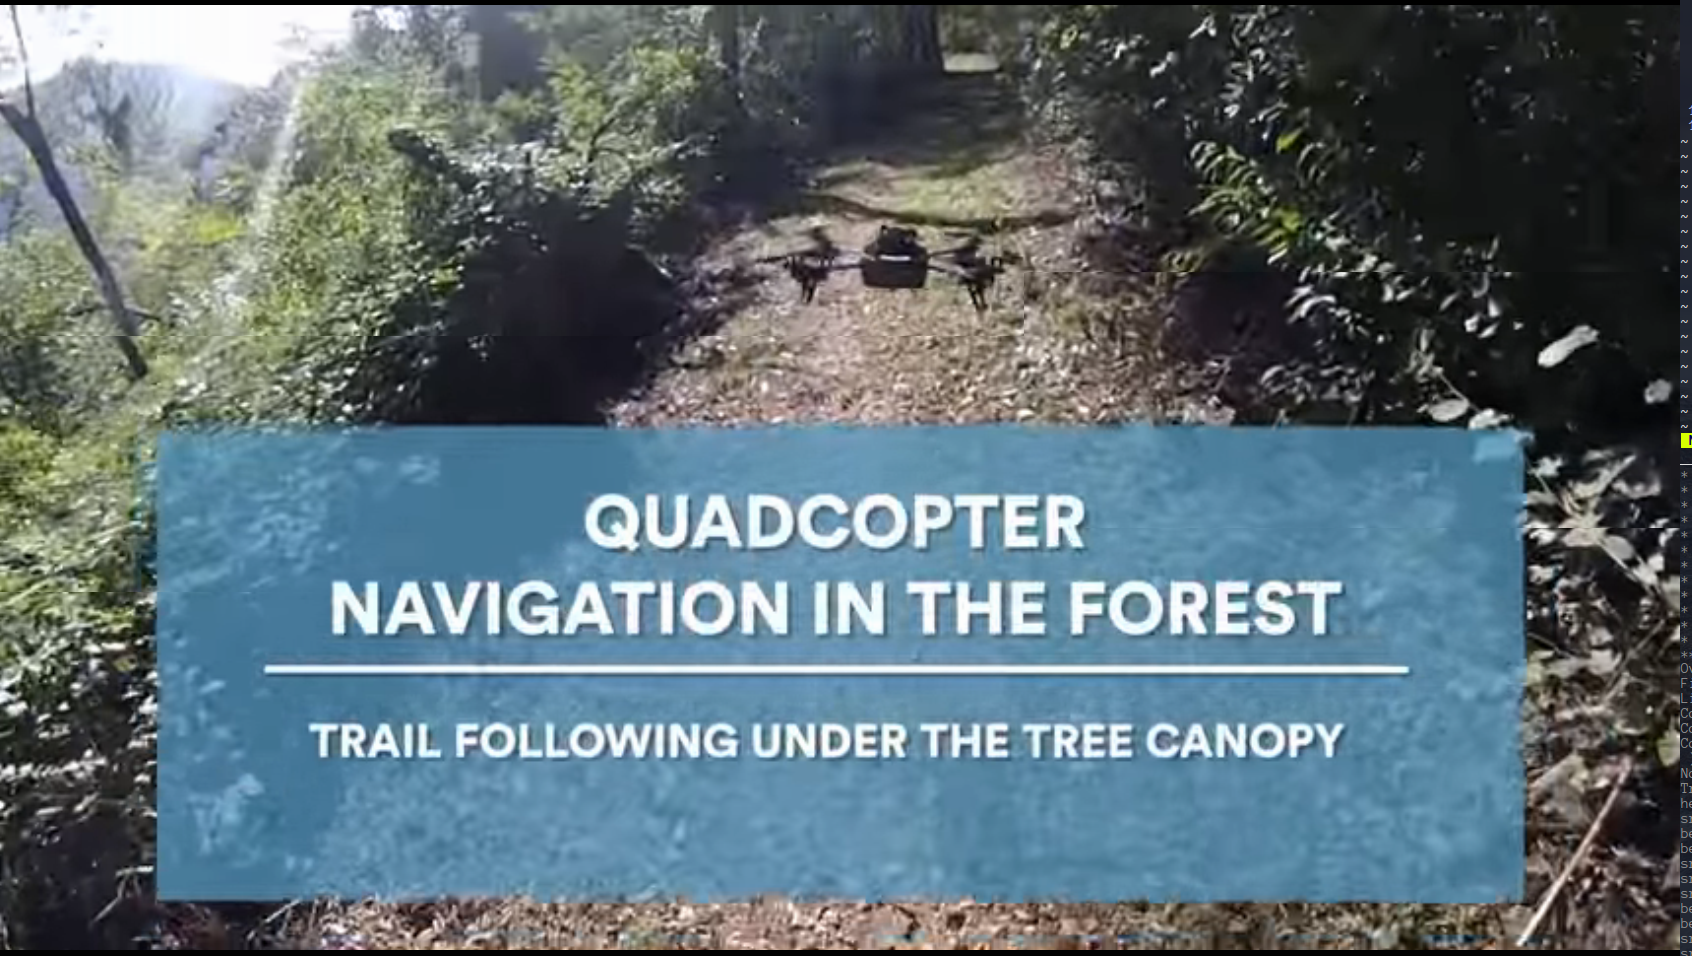
\includegraphics[scale=0.15]{img/quadrotor.png} \\
  	\url{https://www.youtube.com/watch?v=umRdt3zGgpU}
  \end{center}
  \end{frame}
  
  \begin{frame}{Quadrotor im Wald}
  Methodik
  	\begin{itemize}
  		\item Computer Vision
  		\item Deep Neural Network
  		\item Supervised learning
  	\end{itemize}
  \end{frame}
  
  \begin{frame}{Quadrotor im Wald}
  Funktionsweise
  	\begin{itemize}
  		\item Phase 1: Aufnahme des Trails
  		\begin{itemize}
  			\item Drei Kameras um 30° versetzt
  			\item Mittlere Kamera in Richtung des Pfads
  			\item Kategorisierung der Kameras als Links, Mitte und Rechts
  		\end{itemize}
  		\item Phase 2: Das System trainieren
  		\begin{itemize}
  			\item Das System erhält >17.000 Trainingsbilder
  			\item Das System versucht diese in Links, Mitte und Rechts zu kategorisieren
  		\end{itemize}
  		\item Phase 3: Das System testen
  		\begin{itemize}
  			\item Das System wird zuerst mit >7000 Testbildern getestet
  			\item Später: Test auf echten Trails
  		\end{itemize}
  	\end{itemize}
  \end{frame}
  
  \begin{frame}{Quadrotor im Wald}
  	Zusammenfassung
  	\begin{itemize}
  		\item Bei der Kategorisierung ist die Drone stellenweise besser als Menschen
  		\item Die Drone schafft es selbstständig auch auf unbekannten Wegen zu fliegen
  		
  	\end{itemize}
  \end{frame}
  
  %%%%%%%%%%%%%%%%%%%%%%%%%%%%%%%%%%%%%%%%%%%%%%%%
  %%%%%%%%% EUROPA2 %%%%%%%%%%%%%%%%%%%%%%%%%%%%%%
  \section{EUROPA2 - European Robotic Pedestrian Assistant 2.0}
  \begin{frame}{EUROPA2 - European Robotic Pedestrian Assistant 2.0}
  	\begin{center}
  		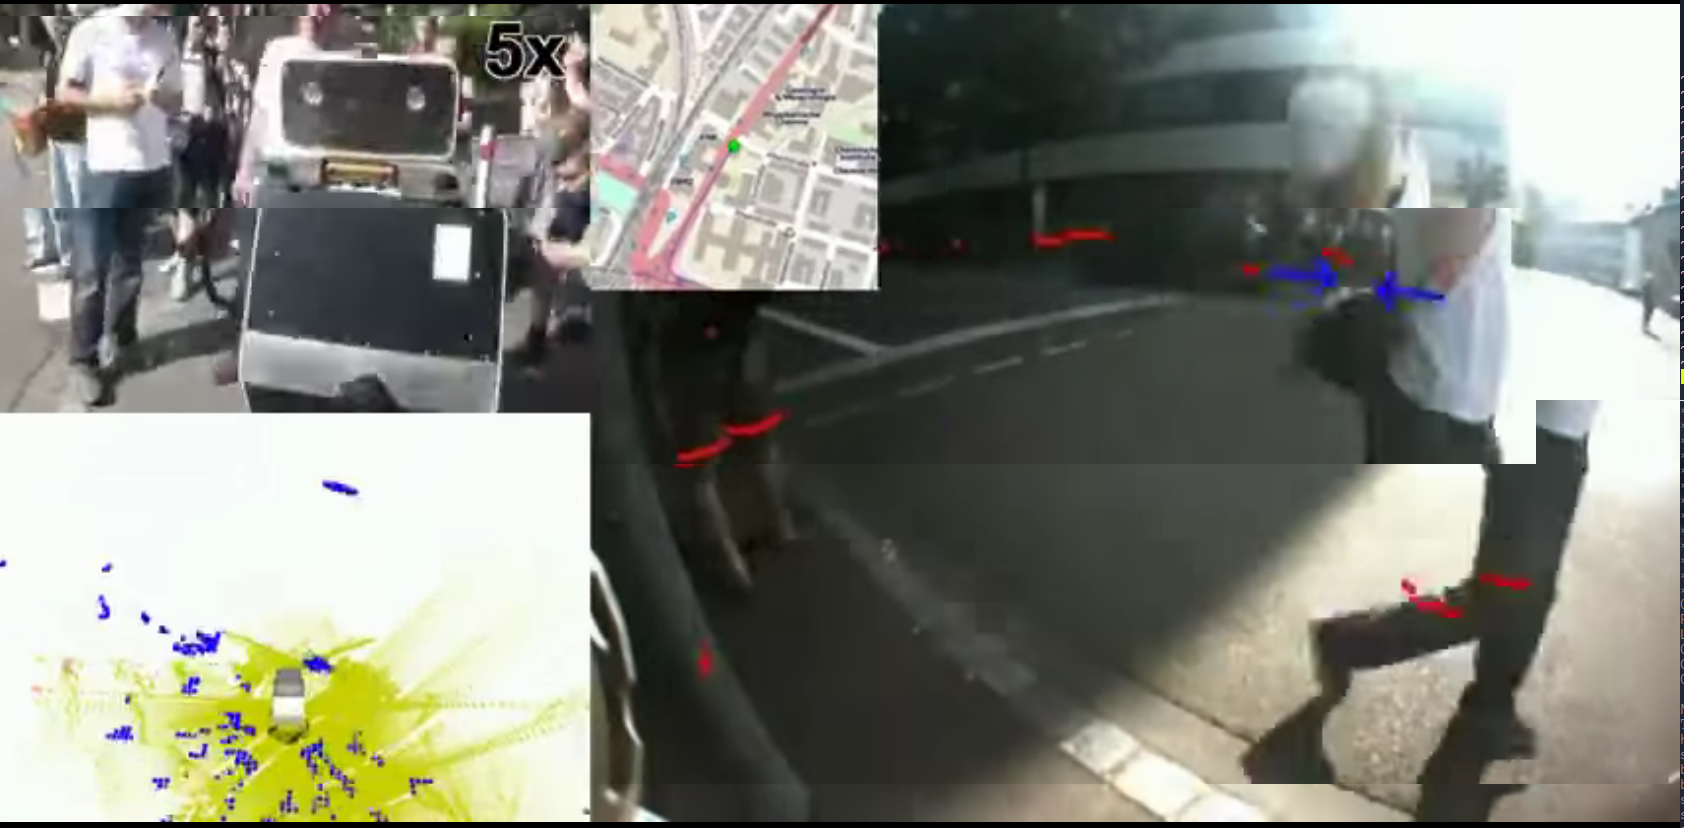
\includegraphics[scale=0.15]{img/europa.png} \\
  		\url{https://youtu.be/A9A29wpkTaU?t=246}
  	\end{center}
  \end{frame}
  
  \begin{frame}{EUROPA2 - European Robotic Pedestrian Assistant 2.0}
  	Es gibt ca 60 Dokumente (Paper und Bücher) zu Themen wie
  	\begin{itemize}
  		% http://europa2.informatik.uni-freiburg.de/files/kretzschmar14icra.pdf
  		\item Vorhersagen zur Bewegung von Menschen
  		% http://europa2.informatik.uni-freiburg.de/files/ilg14icra.pdf
  		\item Rekonstruktion von bewegten Objekten mithilfe eines 2D Laserscanners und einer Kamera
  		% http://europa2.informatik.uni-freiburg.de/files/kuemmerle14jfr.pdf
  		\item Autonome Navigation in populierten Gegenden
  	\end{itemize}
  \end{frame}
  
\end{document}